
\section{Lexicographic Fréchet Distance with Degenerate Inputs}\label{lex_frechet_deg}

\subsection{Problem}

As \citeauthor{rotelex} describes in Section 7 of his paper \citetitle{rotelex} and as we hinted to in Section \ref{sec:lex_frechet_alg} of this paper, multiple critical events can occur for the same $\epsilon$.

Multiple critical events for the same $\epsilon$ turn out to be problematic, because as can be seen in Algorithm \ref{alg:lex_frechet_alg}, we assume the functions defined in Algorithm \ref{alg:lex_frechet_alg_req} return only one critical event, which will be traversed.

This section aims to answer the question of how to handle multiple critical events with the same critical $\epsilon$ by visualizing the problem and postulating an algorithm that decides which combination of critical events result in a lexicographic traversal. The basis of this section is Section 7 of \citeauthor{rotelex}'s paper \citetitle{rotelex}\cite{rotelex}.


\subsection{Examples}

In this subsection, four examples will be discussed, for which multiple critical events for the same critical $\epsilon$ require a decision on which of them should be traversed to result in a lexicographic traversal. Instead of providing in-depth detail on solutions, this subsection aims to illustrate the problem through examples.


\subsubsection{Minimal Example: Traverse Both}
% https://abegehr.github.io/frechet/?p=(5_5)(8_5)(2_5)(5_5)&q=(5.5_3)(4.5_7)

\begin{figure}[H]
    \centering
    
    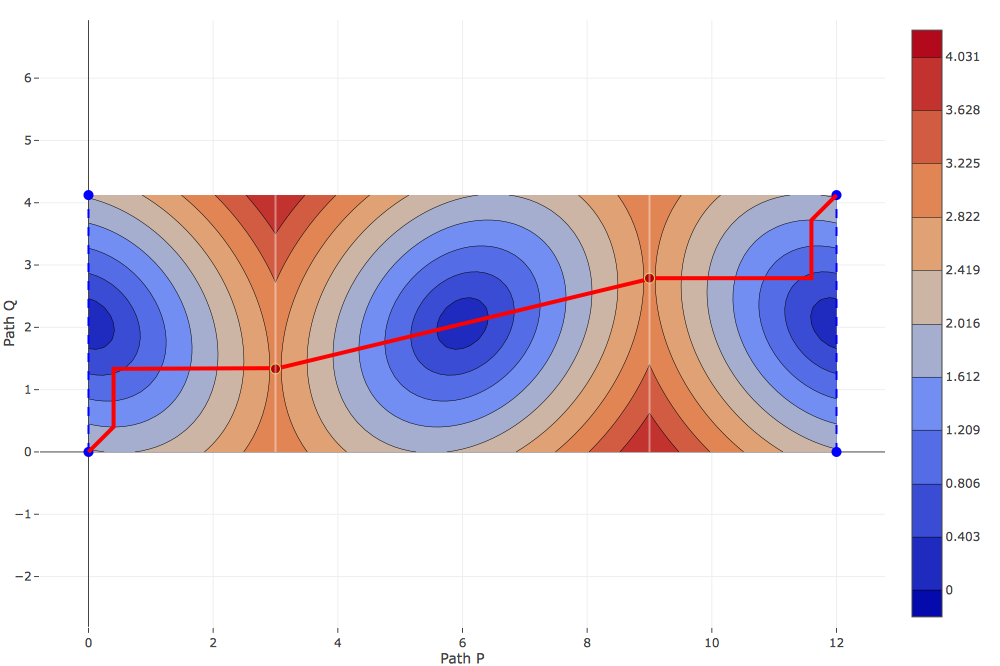
\includegraphics[width=0.8\textwidth]{ces_min_1_tra.png}
		
	\caption{One Path Over Two Critical Events\protect\footnotemark}
    \label{fig:ces_min_1}
\end{figure}
\footnotetext{View the example here: \url{https://abegehr.github.io/frechet/?p=(5_5)(8_5)(2_5)(5_5)&q=(5.5_3)(4.5_7)}}

Figure \ref{fig:ces_min_1} shows a minimal example with two critical events with the same $\epsilon$. There are two classical critical events of type b at $\epsilon \approx 2.91$ at the two vertical cell-borders. Both critical events need to be traversed.


\subsubsection{Minimal Example: Traverse Either}
% https://abegehr.github.io/frechet/?p=(4_5)(8_5)(4_5)&q=(5_4)(5_7)(5_4)

\begin{figure}[H]
    \centering
    
    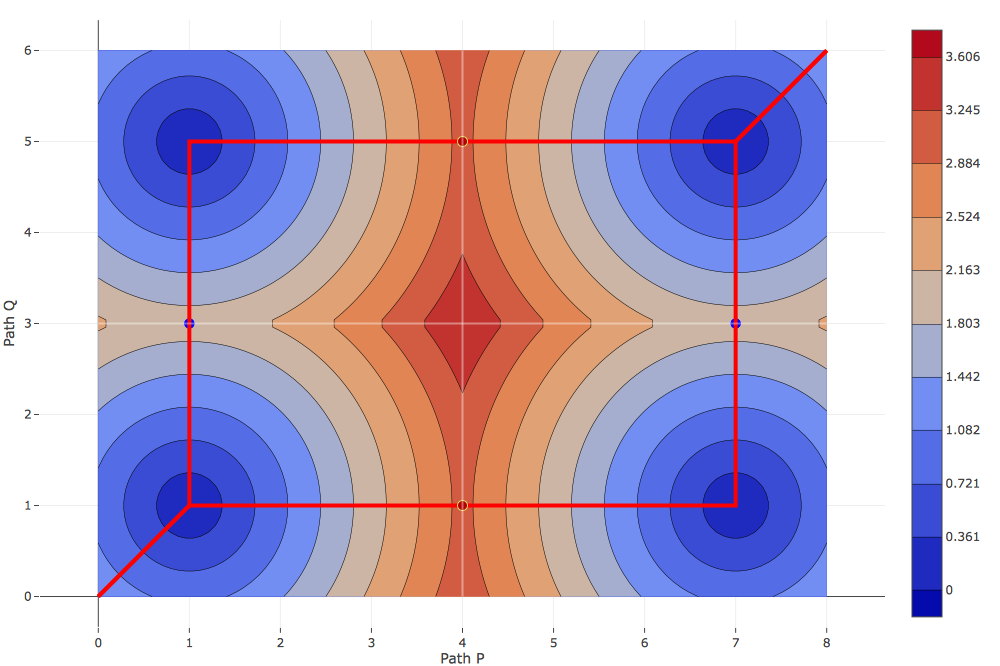
\includegraphics[width=0.8\textwidth]{ces_min_2_tra.png}
		
	\caption{Two Equivalent Paths\protect\footnotemark}
    \label{fig:ces_min_2}
\end{figure}
\footnotetext{View the example here: \url{https://abegehr.github.io/frechet/?p=(4_5)(8_5)(4_5)&q=(5_4)(5_7)(5_4)}}

Figure \ref{fig:ces_min_2} shows a minimal example of multiple critical events for the same $\epsilon$. There are four critical events to consider. Two classical critical events of type b with equal $\epsilon = 3$ at the two vertical cell-borders. And two classical critical events of type b with equal $\epsilon = 2$ at the two horizontal cell-borders. The decision problem shows that $\epsilon = 3$ is needed to traverse this height function $\delta$. Either one of the critical events at $\epsilon = 3$ need to be traversed.



\subsubsection{Minimal Example: Traverse One}
% https://abegehr.github.io/frechet/?p=(3_2)(3_8)(6_4)&q=(2_3)(8_3)(2_3)

\begin{figure}[H]
    \centering
    
    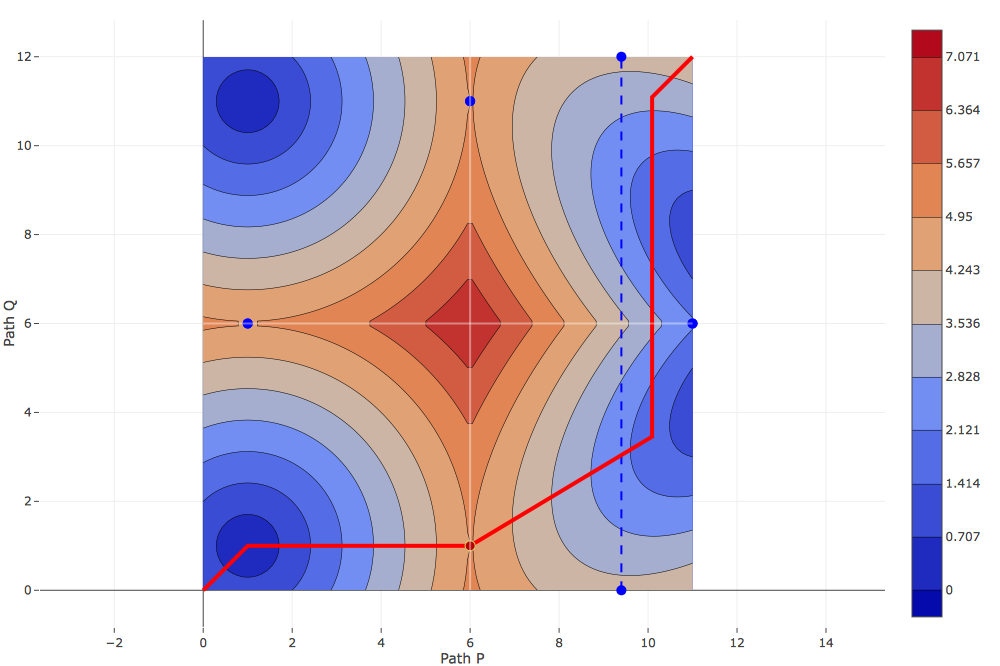
\includegraphics[width=0.8\textwidth]{ces_min_3_tra.png}
		
	\caption{Two Inequivalent Paths\protect\footnotemark}
    \label{fig:ces_min_3}
\end{figure}
\footnotetext{View the example here: \url{https://abegehr.github.io/frechet/?p=(3_2)(3_8)(6_4)&q=(2_3)(8_3)(2_3)}}

Figure \ref{fig:ces_min_3} shows three classical critical events of type b at $\epsilon = 5$ to consider: $C_1(6|1)$, $C_2(1|6)$, and $C_3(6|11)$. There are two possible paths through these three critical events: traversing just $C_1$ or traversing $C_2$ and $C_3$. Since the ascends to and descends from $C_1$, $C_2$, and $C_3$ are similar, we choose the path over only $C_1$.



\subsubsection{Complex Example}

Figure \ref{fig:ces_com} shows a more complex example of multiple critical events for the same $\epsilon$. 






\subsection{Possible Paths}

We have seen in the examples, that in some cases we need to traverse a path through multiple of the critical events at equal height $\epsilon_0$, while in other cases a path through one critical events is sufficient. To decide which path to traverse, first, we need to find all possible paths through the critical events.

The possible paths through multiple critical events can be represented as a graph. The start node represents the lower left corner $A$ and the end node represents the upper right corner $B$ of the current $\delta$ subsection. Each critical event $C_k \in C$ of height $\epsilon_0$ is a node. Edges are directional and denote traversability without another critical event of height $\epsilon_0$ in between.

To generate this graph of critical traversals, we make use of the free-space diagram and the technique used in the decision algorithm. Fist we use the free-space diagram represented by $L_{ij}^F$ and $B_{ij}^F$ and the decision algorithm (see \citet{altgodau}) to generate the reachable border bounds $L_{ij}^R$ and $B_{ij}^R$ of all cells. Then we use the reachable border bounds and the critical events $C$ at height $\epsilon_0$ to generate for each vertical and horizontal cell-border, which subset of critical events $C$ can reach the border. We call the subset of $C$, that reaches the left and bottom border of cell $(i,j)$, $L_{ij}^C$ and $B_{ij}^C$ respectively. After computing each $L_{ij}^C$ and $B_{ij}^C$, we then connect critical events in $L_{ij}^C$ and $B_{ij}^C$ to reachable critical events starting on the top and right border.

See the algorithm \ref{alg:gengraph} for more detail on how we generate the traversability graph of multiple critical traversals $C_k$ that are at same height $\epsilon_0$. $p$ and $q$ is the number of cells between the starting-point $A$ and the ending-point $b$.


\begin{algorithm}[H]
\caption{Generate Traversability Graph of multiple critical events at $\epsilon_0$}\label{alg:gengraph}
\begin{algorithmic}[1]

\Function{GenerateTraversalGraph($A, B, C, \epsilon_0$)}{}
	\State\Comment{$A$ is start-point of traversal. $B$ is ending-point of traversal. $C$ holds all critical events $C_k$.}
	
	\State {Add $A$ and $B$ as critical events to $C$.}

	\State {$\forall i,j: L_{ij}^C := \{\} \wedge B_{ij}^C := \{\}$}
	
	\State $L^R, B^R \gets$ \Call{DecisionAlgorithm'}{$A, B, \epsilon_0$}

	\For {$C_k \in C$}
		\State {Add $C_k.B$ (ending-points) to $L_{ij}^C$ or $B_{ij}^C$ where $C_k.B$ lies.}
	\EndFor

	\For {$i := 0$ to $p$} {determine $L_{i, 0}^C$} \EndFor
	\For {$j := 0$ to $q$} {determine $B_{0,j}^C$} \EndFor
	 
	\For {$i := 0$ to $p$}
		\For {$j := 0$ to $q$}
			
			\For {$C_{k2}$ that starts on right or top border}
				\For {$C_{k1} \in L_{i, j}^C \cup B_{i, j}^C$}
					
					\If {$C_{k1}$ can reach $C_{k2}$} \label{alg:gengraph_reach}
						\State {Add edge $(C_k1$, $C_k2)$ to graph.}
					\EndIf
					
				\EndFor
			\EndFor
			
			\State {construct $L_{i+1, j}^C$ and $B_{i, j+1}^C$ from $L_{ij}^C$, $B_{ij}^C$, $L_{i+1, j}^R$, $B_{i, j+1}^R$}
		
		\EndFor
	\EndFor
	
	\Return {graph}

\EndFunction

\end{algorithmic}
\end{algorithm}

\subsubsection{Can $C_{k1}$ reach $C_{k2}$}

In the above algorithm \ref{alg:gengraph} on line \ref{alg:gengraph_reach}, we seek to determine if the critical event $C_{k1}$ can reach the critical event $C_{k2}$. It is known that $C_{k1}$ can reach the left or bottom border of the current cell $(i, j)$, because $C_{k1} \in L_{i, j}^C \cup B_{i, j}^C$. It also is know that $C_{k2}$ starts at the top or right border of the current cell.

We discard the potential edge $(C_{k1}, C_{k2})$ in the trivial case where $C_{k2}$ is not monotonically reachable from $C_{k1}$: $\neg(C_{k1}.B.x \leq C_{k2}.A.x \wedge C_{k1}.B.y \leq C_{k2}.A.y)$.

To determine if $C_{k2}$ is reachable from $C_{k1}$, we first look at if $C_{k1}$ comes the left or bottom border and if $C_{k2}$ is on the right or top border. There are four cases to consider:

\begin{enumerate}
	\item $C_{k1} \in L_{i, j}^C$ enters on left border and $C_{k2}$ starts on right border.
	\item $C_{k1} \in L_{i, j}^C$ enters on left border and $C_{k2}$ starts on top border.
	\item $C_{k1} \in B_{i, j}^C$ enters on bottom border and $C_{k2}$ starts on right border.
	\item $C_{k1} \in B_{i, j}^C$ enters on bottom border and $C_{k2}$ starts on top border.
\end{enumerate}

Reachability intervals $I_{ij}$ of right and top borders can be computed as follows:

\begin{enumerate}
	\item From left to right: $I_{ij}^{l \rightarrow r} = L_{i, j}^R \cap L_{i+1, j}^R$
	\item From left to top: If $L_{i, j}^R$ is open: $I_{ij}^{l \rightarrow t} = B_{i, j+1}^R$. Otherwise closed.
	\item From bottom to right: If $B_{i, j}^R$ is open: $I_{ij}^{b \rightarrow r} = L_{i+1, j}^R$. Otherwise closed.
	\item From bottom to top: $I_{ij}^{b \rightarrow t} = B_{i, j}^R \cap B_{i, j+1}^R$
\end{enumerate}

The superscript denotes the sides of the cell. $I_{ij}^{b \rightarrow t}$ for example represents the reachability interval of the top border for traversals coming from the bottom border.

It can be considered to use solely these reachability intervals $I_{ij}$ to decide if $C_{k2}$ can be reached from $C_{k1}$. One would simply check if $C_{k2}$ lies in the reachability intervals from the side on which $C_{k1}$ lies. This is not sufficient, as the example visualized in figure \ref{fig:gengraph_ex1} shows.

\begin{figure}[H]
    \centering
    
    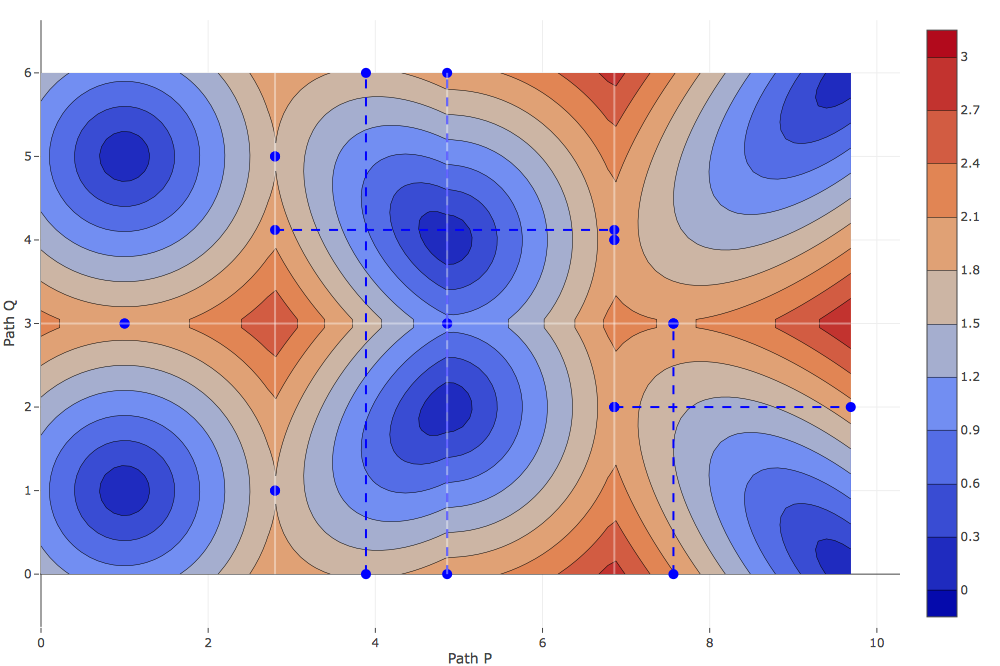
\includegraphics[width=0.8\textwidth]{gengraph_ex1.png}
		
	\caption{Considering solely reachability intervals is not sufficient\protect\footnotemark}
    \label{fig:gengraph_ex1}
\end{figure}
\footnotetext{View the example here: \url{https://abegehr.github.io/frechet/?p=(5_5)(5_7.8)(4_6)(4_8)(6_6)&q=(6_6)(3_6)(6_6)}}

In figure \ref{fig:gengraph_ex1} the decision algorithm tells us, that the classical Fréchet distance is $\epsilon_F = 2$. There are two critical events of type b with $\epsilon = 2$ that we consider: $C_1(3, 1)$ and $C_2(\sim6.86, 4)$. If we were to use solely the reachability intervals to check if $C_{k2}$ is reachable from $C_{k1}$ as described above, the generated graph would find an edge between $C_1$ and $C_2$, even though there exists no such path, because it is closed by the right border of cell $(0, 1)$: $L_{1, 1}^R$. Using solely the reachability intervals, $C_2$ would still appear reachable from $C_1$, because $L_{2, 1}^R$ starts below $L_{1, 1}^R$, since $L_{2, 1}^R$ can also be reached from $B_{1,1}^R$, and not just from $L_{1, 1}^R$. We can now learn from this counter example and apply better measures.

To solve the problem of reachability intervals for generating a traversability graph of critical events, we need to memorize for each critical event not just that it can reach border $L_{ij}$ or $B_{ij}$, but also for vertical borders the minimum $y$-coordinate and for horizontal borders the minimum $x$-coordinate that it needs to reach the border, as these can differ for different critical events that both reach a border. Then when we connect a critical event $C_{k1}$ to $C_{k2}$, we test the reachability intervals and we determine if the $C_{k2}$ lies on or above the minimum $x$- or $y$-coordinate that $C_{k1}$ needs to reach the border in question.

We can now define two algorithm in more detail. First, the algorithm for determining if $C_{k1}$ can reach $C_{k2}$. And second, the algorithm that constructs $L_{i+1, j}^C$ and $B_{i, j+1}^C$ from $L_{ij}^C$, $B_{ij}^C$, $L_{i+1, j}^R$, $B_{i, j+1}^R$.

\begin{algorithm}[H]
\caption{Generate Traversability Graph Helper Functions}\label{alg:gengraph_help}
\begin{algorithmic}[1]

\Function{CanReach($C_{k1}, min_{x}, min_{y}, C_{k2}, I_{ij}^{l \rightarrow r}, I_{ij}^{l \rightarrow t}, I_{ij}^{b \rightarrow r}, I_{ij}^{b \rightarrow t}$)}{}
	\State\Comment{Determines if $C_{k1}$ can reach $C_{k2}$.}
	
	\If {$C_{k1}$ is on left border and $C_{k2}$ is on right border}
		\State\Return {$C_{k2}.A.y \in I_{ij}^{l \rightarrow r} \wedge C_{k2}.A.y \geq min_{y}$}
	\EndIf
	\If {$C_{k1}$ is on left border and $C_{k2}$ is on top border}
		\State\Return {$C_{k2}.A.x \in I_{ij}^{l \rightarrow t} \wedge C_{k2}.A.x \geq min_{x}$}
	\EndIf
	\If {$C_{k1}$ is on bottom border and $C_{k2}$ is on right border}
		\State\Return {$C_{k2}.A.y \in I_{ij}^{b \rightarrow r} \wedge C_{k2}.A.y \geq min_{y}$}
	\EndIf
	\If {$C_{k1}$ is on bottom border and $C_{k2}$ is on top border}
		\State\Return {$C_{k2}.A.x \in I_{ij}^{b \rightarrow t} \wedge C_{k2}.A.x \geq min_{x}$}
	\EndIf
\EndFunction

\State

\Function{ConstructCriticalReach($L_{ij}^C$, $B_{ij}^C$, $L_{i+1, j}^R$, $B_{i, j+1}^R$)}{}
	\State\Comment{Constructs $L_{i+1, j}^C$ and $B_{i, j+1}^C$ from $L_{ij}^C$, $B_{ij}^C$, $L_{i+1, j}^R$, $B_{i, j+1}^R$}
	
	\State {$L_{i+1, j}^C := \{\}$}
	\State {$B_{i, j+1}^C := \{\}$}
	
	\If {$L_{i+1, j}^R$ is not closed}
		\For {$(C_k, min_{x}) \in B_{ij}^C$}
			\State {Add $(C_k, L_{i+1, j}^R.min)$ to $L_{i+1, j}^C$}
		\EndFor
		\For {$(C_k, min_{y}) \in L_{ij}^C$}
			\If {$min_{y} \leq L_{i+1, j}^R.max$}
				\State {$min_{y} \gets max(min_{y}, L_{i+1, j}^R.min$)}
				\State {Add $(C_k, min_{y})$ to $L_{i+1, j}^C$}
			\EndIf
		\EndFor
	\EndIf
	
	\If {$B_{i, j+1}^R$ is not closed}
		\For {$(C_k, min_{y}) \in L_{ij}^C$}
			\State {Add $(C_k, B_{i, j+1}^R.min)$ to $B_{i, j+1}^C$}
		\EndFor
		\For {$(C_k, min_{x}) \in B_{ij}^C$}
			\If {$min_{x} \leq B_{i, j+1}^R.max$}
				\State {$min_{x} \gets max(min_{x}, B_{i, j+1}^R.min$)}
				\State {Add $(C_k, min_{x})$ to $B_{i, j+1}^C$}
			\EndIf
		\EndFor
	\EndIf
	
	\State\Return {$L_{i+1, j}^C, B_{i, j+1}^C$}
	
\EndFunction

\end{algorithmic}
\end{algorithm}

The two functions defined in algorithm \ref{alg:gengraph_help} are necessary for algorithm \ref{alg:gengraph} to generate the correct traversability graph for a set of critical events at the same height $\epsilon_0$.

It might be that it is superfluous to check if $C_{k2}.A$ lies in the respective reachability interval, because we are checking for the minimum $x$- or $y$-coordinate. Nevertheless, also checking the reachability interval $I_{ij}$ does not hurt the valid functioning.


\subsection{Whut}

To fulfill our goal of a lexicographic traversal, we want to minimize the time during which the height $\epsilon$ exceeds a threshold.\cite{rotelex} Concerning our example, we want to minimize the time needed to ascend to and descend from our critical height $\epsilon = 5$. 

For a critical event $C_i$, we will denote the ascent with $C_i^\uparrow$ and descent with $C_i^\downarrow$.

We will now calculate the ascents $C_1^\uparrow$, $C_2^\uparrow$, and $C_3^\uparrow$ as well as the descents $C_1^\downarrow$, $C_2^\downarrow$, and $C_3^\downarrow$, taking the steepest (monotonic) descent in all six cases.


\subsection{Postulate Algorithm}
Postulate algorithm for choosing a critical event from several with equal epsilon: (visual examples!)

Algorithm:
\begin{enumerate}
	\item For every critical event compute reciprocal of derivates descents and store as critical event's steepness.
	\item From set of critical events, generate all possible sequences (ascending monotone).
	\item For all sequences sum steepness of their critical events and store as sequence rank.
	\item Starting with the smallest-rank sequence, decide if the sequence of critical events is traversable without passing critical events excluded in the sequence.
	\item If decision is negative, repeat 4.
	\item If decision is positive, repeat 4 for all sequences of equal rank.
	\item If multiple sequences of equal rank are found to be valid, traverse all, and decide by comparing.
	\item The steepness of the steepest decent.
	\item The steepness of critical event that is reached.
	\item And choose the path with the steepest summed recents of all paths.
	\item If multiple paths with same hight profile are found, return all. Otherwise return the lexicographic optimum.
	\item 
\end{enumerate}

\subsection{Traversing critical events}

Assume we are traversing a heat map generated by two curves. We arrive at a point where we have to decide which critical events need to be traversed for a lexicographic solution. The decision algorithm\cite{altgodau} can be applied for the $\epsilon$ of each possible critical event. We pick the smallest $\epsilon$ for which the decision algorithm returns a positive decision. We call it $\epsilon_0$. Now two options are feasible:

\begin{enumerate}[label=(\Alph*)]
	\item There is one critical event at height $\epsilon_0$. $|C_{\epsilon_0}| = 1$
	\item There are multiple critical events at height $\epsilon_0$. $|C_{\epsilon_0}| > 1$
\end{enumerate}

In case option A holds true, this critical event will need to be traversed. The traversal-problem is divided into two sub problems, which are both examined recursively and independently.

In case option B holds true, we need to decide which of the critical events $C_{\epsilon_0}$ need to be traversed and which are not needed for an optimal solution. We will consider all subsets $C'_{\epsilon_0}$ of $C_{\epsilon_0}$ with size $n>0$.

\subsubsection{Traversing multiple critical events with same $\epsilon$}

For each subset of critical events at $\epsilon_0$, $C'_{\epsilon_0} \subseteq C_{\epsilon_0}$ we compute if the critical events can be traversed monotonic. This can be done easily by applying the following procedure. For each critical event $C'_{\epsilon_0}(i)$, test if the start- and ending-points of all other critical events in $C'_{\epsilon_0}$ are either lower-left of the starting point of $C'_{\epsilon_0}(i)$ or upper-right of the ending point of $C'_{\epsilon_0}(i)$.

See the a pseudocode for the function here. The function will return $True$ if the critical events $C'_{\epsilon_0}$ are traversable monotonically and $False$ if they are not.
\begin{algorithm}[H]
\caption{Critical Events $C'_{\epsilon_0}$ Monotonic Traversable}\label{euclid}
\begin{algorithmic}[1]

\Function{$PLeq(p, q)$}{}
	\State \Comment{determines if two points are monotonically traversable}
	\State \Return {($p_x \leq q_x$ \textbf{and} $p_y \leq q_y$)}
\EndFunction

\State {}

\Function{MonotonicTraversable($C'_{\epsilon_0}$)}{}
	\State \Comment{Determines if a set of critical events $C'_{\epsilon_0}$ are monotonically traversable.}
	
	\For {i in len($C'_{\epsilon_0}$)}
		\State $c_{i} \gets C'_{\epsilon_0}(i)$
		\State $c_{i,s} \gets c_{i}.start$
		\State $c_{i,e} \gets c_{i}.end$
		\State {}
	
		\For {j in len($C'_{\epsilon_0}$)}
			\If {$j == i$}
				\textit{continue}
				\Comment{$c_{j}$ is skipped} \EndIf
			\State {}
			
			\State $c_{j} \gets C'_{\epsilon_0}(j)$
			\State $c_{j,s} \gets c_{j}.start$
			\State $c_{j,e} \gets c_{j}.end$
			\State {}
			
			\If {$PLeq(c_{j,s}, c_{i,s})$ \textbf{and} $PLeq(c_{j,e}, c_{i,s})$}
				\State \textit{continue}
				\Comment{$c_{j}$ is traversable prior to $c_{i}$}
			\EndIf
			\If {$PLeq(c_{i,e}, c_{j,s})$ \textbf{and} $PLeq(c_{i,e}, c_{j,e})$}
				\State \textit{continue}
				\Comment{$c_{j}$ is traversable after $c_{i}$}
			\EndIf
			\State {}
				
			\State \Return $False$ \Comment{$c_{i}$ and $c_{j}$ are not traversable monotonically}
		\EndFor
	\EndFor
	\State \Return $True$ \Comment{the critical events $C'_{\epsilon_0}$ are monotonically traversable}
\EndFunction
\end{algorithmic}
\end{algorithm}

$MonotonicTraversable$ is applied to all subsets of critical events at $\epsilon_0$, $C'_{\epsilon_0} \subseteq C_{\epsilon_0}$. We will only consider the critical events $C'_{\epsilon_0}$, for which $C'_{\epsilon_0}$ is monotonically traversable, \textit{i.e.} $MonotonicTraversable(C'_{\epsilon_0})$ holds True, because other combinations of critical events are not monotonically traversable. We call this monotonically traversable subset $C''_{\epsilon_0} \subseteq C_{\epsilon_0}$ .

$$ C''_{\epsilon_0} \coloneqq \{ C'_{\epsilon_0} \mid MonotonicTraversable(C'_{\epsilon_0}) \} $$



\subsection{Example of Algorithm visualised (visual example!)}

\subsection{Analysing postulated algorithm for handling degenerate inputs}
\subsubsection{Runtime analysis}
\subsection{Real world application}
	Can you think of one?
	
	
	
	